\section*{Источники и решения}

\subsubsection*{Монеты на столе}

Эта интересная головоломка досталась мне от специалиста по информатике Гая Киндлера во время чудесного года, проведённого нами в принстонском Институте перспективных исследований.

\begin{figure}[t!]
\centering
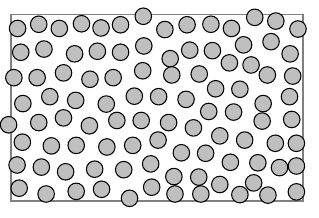
\includegraphics[scale=1]{pics/coin1}
\caption{Нельзя добавить новую монету без перекрытия со старыми.}
\label{pic:coin1}
\end{figure}

\begin{figure}[b!]
\centering
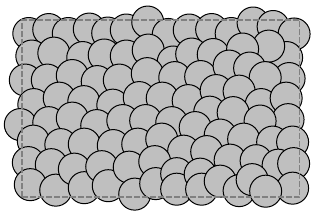
\includegraphics[scale=1]{pics/coin2}
\caption{Стол покрыт удвоенными монетами.}
\label{pic:coin2}
\end{figure}

Начнём с того, что если удвоить радиус каждой монеты (скажем, с $1$ до $2$), то как видно на рисунках \ref{pic:coin1} и \ref{pic:coin2}, покроется весь стол.
Почему?
Ну если какая-то точка $P$ не покрыта, то она лежит на расстоянии $2$ или более от центра любой монеты, так что к исходной конфигурации можно было добавить (маленькую) монету, с центром в $P$.

Дело было бы сделано, если бы большая монета покрывалась четырьмя маленькими.
Однако это не так.

Тем не менее нужным свойством обладает \emph{сам} прямоугольник --- он разбивается на четыре уменьшенные копии самого себя.
Итак, сожмём вдвое всю картинку (рис. \ref{pic:coin2}, где большие монеты покрывают весь стол) и воспользуемся четырьмя её копиями (как на рис. \ref{pic:coin3}).
Так мы покроем весь исходный стол!


\begin{figure}[t!]
\centering
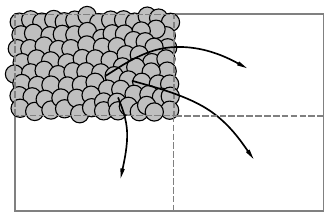
\includegraphics[scale=1]{pics/coin3}
\caption{Четыре уменьшенные стола покрывают стол целиком.}
\label{pic:coin3}
\end{figure}

\medskip

Это красивое рассуждение, выглядит грубым, однако (как ни странно) оно даёт наилучшую оценку --- замените $4$ на что-то меньшее, скажем, $3{,}99$, и полученное утверждение перестанет быть верным.

Чтобы это понять, рассмотрим предельный случай, когда стол очень большой, а монет так много, что граничные эффекты пренебрежимо малы.
Заменим стол на пол ванной комнаты, покрытый мозаикой в виде пчелиных сот;
то есть каждая плитка это правильный шестиугольник диаметра (скажем) 2.
Сама плитка имеет площадь $6\times\sqrt{3}/4=3\times\sqrt{3}/2$, ведь каждая плитка разбивается на шесть равносторонних треугольников со стороной 1 и, значит, площади $\sqrt{3}/4$.

\begin{figure}[t!]
\centering
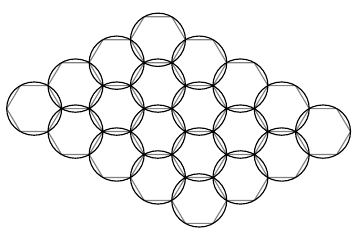
\includegraphics[scale=1]{pics/coin4}
\caption{Покрытие описанными кругами правильных шестиугольников.}
\label{pic:coin4}
\end{figure}

\begin{figure}[b!]
\centering
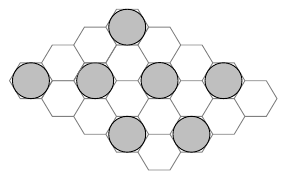
\includegraphics[scale=1]{pics/coin5}
\caption{Разряженная конфигурация.}
\label{pic:coin5}
\end{figure}

Весь пол можно покрыть, положив на каждую плитку монету, граничная окружность которой описана вокруг плитки (см. рис. \ref{pic:coin4}).

Тогда каждая монета имеет радиус $1$ и, следовательно, площадь~$\pi$.
Если $A$ --- площадь всего пола, то, игнорируя граничные эффекты, общая площадь монет будет $\pi A/(3\sqrt{3}/2)\sim 1{,}2092\times A$.

Теперь разберёмся, насколько разрежённо можно расположить монеты на полу, чтобы нельзя было добавить новую монету без перекрытия со старыми.
Воспользуемся той же плиткой, но на этот раз покроем только треть плиток (рис. \ref{pic:coin5}).
В середину каждой такой плитки положим по монете с радиусом чуть больше радиуса вписанной в шестиугольник окружности. 
Это не позволит добавлять монет.

Какова же площадь всех этих монет?

Радиус монеты чуть больше высоты одного из шести равносторонних треугольников, составляющих шестиугольник — а именно, $\sqrt{3}/2$.
Следовательно, площадь монеты чуть превысит $\pi \z\times (\sqrt{3}/2)^2 \z= 3\pi/4$.

Отсюда следует, что общую площадь монет на полу можно сделать произвольно близкой к $(1/3) \times (3\pi/4) \times A/(3\sqrt{3}/2) = \pi A/(6 \sqrt{3}) \z\sim 0{,}3023 \times A$, а это ровно четверть того, что было раньше!

\medskip

Мы не только решили головоломку, но и доказали пару экстремальных свойства кругов.

Первое утверждает, что нет лучшего способа покрыть плоскость единичными кругами, чем описать круги вокруг плиток шестиугольной мозаики, как мы сделали выше.
Второе, --- что нет более разреженной конфигурации монет \emph{без} возможности добавить лишнюю, чем помещать на каждой третьей плитке круг, чуть больший, чем вписанный, опять же, как мы проделали выше.

Если вам эти свойства очевидны, то подумайте о следующем ещё более очевидном утверждении: \emph{самая плотная упаковка единичных кругов на  плоскости получается из кругов, вписанных в шестиугольники пчелиных сот}.
Это было доказано только в 1972 году видным венгерским геометром Ласло Фейешем Тотом (1915---2005)!

\begin{addedbytheeditors}
Доказательства всех трёх последних утверждений приводятся в замечательной книжке Фейеша Тота \cite[III §3]{tot}.
Конечно же все они были доказаны раньше публикации немецкого оригинала книги в 1953 году, а никак не в 1972 году!
Приведённые в решении аргументы на примере двумерного случая иллюстрируют связь между двумя фундаментальными задачами геометрии чисел --- проблемой упаковки шаров и задачей о покрытии пространства перекрывающимися шарами. Подробности на эту тему см. в книге Джона Конвея и Нила Слоэна \cite{conway-sloane}. 
%Все они связаны с так называемой задачей упаковки шаров, которая обсуждается в книге Джона Конвея и Нила Слоэна \cite{conway-sloane}.
%У задачи про монеты есть две вариации. Они отличаются тем, что связывают между собой упаковки (в первом случае) и покрытия (во втором) кругами разных радиусов. 
%Если на прямоугольный противень помещается $100$ печений радиуса $2$, то  на такой же противень поместится и $400$ печений радиуса $1$.
%Если прямоугольник можно заклеить (без просветов, но разрешается вылезать за пределы) $100$ кругами радиуса $2$, то его можно заклеить и $400$ кругами радиуса $1$.
%А: Я это закоментил потому как это просто переформулировка промежуточниого результата. 
%+ если есть причина восстанавливать этот текст, то назовите её --- по-моему он ровно ничего не добавляет.
\pr
\end{addedbytheeditors}

\subsubsection*{Четыре точки с двумя расстояниями}

Эта замечательная головоломка годится для болтовни за обедом;
она была включена в раздел головоломок журнала «Pi Mu Epsilon» \cite[1985 год, задача 3a, предложена Ш. Дж. Эйнхорном и И. Дж. Шёнбергом]{16}.
Позже появилась на первой странице книги Ноба Ёсигахары \cite{61}, где была приписана Дику Хессу.

Я заметил, что очень мало людей находят все шесть конфигураций;
почти каждый упирается в какое-то препятствие или совершает ошибку, пропуская одну из них.
При этом непредсказуемо, \emph{какую} именно; один из испытуемых упустил квадрат!

\begin{figure}[ht!]
\centering
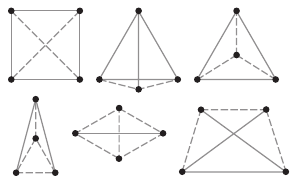
\includegraphics[scale=1]{pics/2dist}
\caption{Все шесть вариантов.}
\label{pic:2dist}
\end{figure}

Все конфигурации показаны на рис. \ref{pic:2dist}.
Последняя из них (трапеция) образована четырьмя вершинами правильного пятиугольника.


\subsubsection*{Преступница и собака}

Моё внимание к этой интересной задаче привлёк Хулио Дженовезе;
она появилась в книге Мартина Гарднера \cite{24}.

Будем считать, что круг имеет единичный радиус.
Представим, что преступница бегает в меньшем концентрическом круге радиуса $r$, где $r < \tfrac14$.
Тогда она сможет попасть в точку круга, которая находится на максимальном расстоянии от собаки (см. рис. \ref{pic:dog}).
Это потому, что длина окружности меньшего круга составляет меньше четверти длины забора.

Если $r$ достаточно близко к $\tfrac14$, то преступница может бежать прямо к забору.
Это расстояние чуть больше чем $3/4$, а собаке придётся пробежать пол окружности поля, то есть $\pi$.
Так как $\pi > 3$, это более чем в четыре раза превысит путь преступницы.

\begin{figure}[h!]
\centering
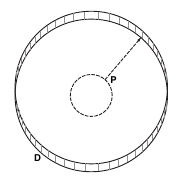
\includegraphics[scale=1]{pics/dog}
\caption{Точка, из которой преступница бежит к забору.}
\label{pic:dog}
\end{figure}

Преимущество собаки в скорости можно увеличить с $4$ до $4{,}6033388$; при этом лучшая стратегия обеих сторон приведёт к тому, что они финишируют одновременно.
Больше информации об этой задаче  можно найти на сайте головоломок IBM «Ponder This» за \cite[май 2001]{ponder-this}.

\subsubsection*{Теннисная загадка}

На этот недочёт указал мне Дик Хесс --- знаток головоломок и тенниса.
На рис. \ref{pic:tenis} показано место приземления мяча; и это ошибка при подаче --- мяч не задевает «коробку» подачи, но при этом задевает две линии линейных судей. 
Использование электронных систем контроля задней линии не помогает.
Интересно бы выяснить, часто ли такая подача ошибочно засчитывается.

\begin{figure}[ht!]
\centering
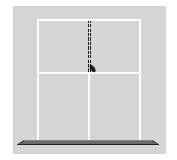
\includegraphics[scale=1]{pics/tenis}
\caption{Кто должен увидеть эту ошибку при подаче?}
\label{pic:tenis}
\end{figure}


\subsubsection*{Двойное покрытие прямыми}


Некоторых читателей это разочарует, но ответ да (если принять аксиому выбора), и есть уйма способов это сделать. 
Однако доказательство требует трансфинитной индукции (!), не оставляя места геометрии.
Задачу (и её решение) мне подбросил физик Сеня Шлосман, который не знает её происхождения.

Данное решение мне нравится как пример простого применения мощного инструмента.
Идея в следующем: мы начинаем с трёх пересекающихся прямых, так что у нас уже есть три направления.
Пусть $\kappa$ --- наименьший ординал мощности континуум (то же, что множество точек на прямой, точек на плоскости или углов на плоскости).
Посмотрим на множество ординалов ниже $\kappa$.
Каждый из них --- либо последовательный ординал (как, например, $17$, $188$ или $\omega + 1$), либо предельный ординал (как, например, $\omega$, первый бесконечный ординал); у каждого мощность строго меньше континуума.
Мощность ординалов ниже $\kappa$ --- континуум, поэтому этими ординалами можно пометить все точки плоскости.
Теперь точки плоскости образуют \emph{вполне упорядоченное} множество, то бишь каждое непустое подмножество содержит точку с минимальной меткой.

Приступим к трансфинитной индукции.
Предположим, у нас есть конфигурация прямых, покрывающая все точки множества точек $S$ с метками меньше $\sigma$ ровно дважды,
точка $P$ с меткой $\sigma$ покрыта менее двух раз,
и ни одна из точек плоскости не покрыта три раза или более.
Напомним, что $\sigma$ --- ординал, меньший $\kappa$.
Можно считать, что каждая прямая в конфигурации проходит через одну из точек множества $S$, и, значит, прямых в конфигурации меньше чем континуум.
Значит, и мощность всех двойных точек конфигурации меньше континуума.
Так как множество направлений прямых континуально, через точку $P$ можно провести прямую, не проходящую через двойные точки,
то есть её можно добавить к нашей конфигурации.
Если $P$ всё ещё не двойная, то придётся повторить ещё один раз.

Похоже на обман?
Ну да; наше построение совсем не конструктивно.
Означает ли это, что \emph{не существует} хорошего построения двойного покрытия?
Нет, но я такой пример найти не смог; не смог и Сеня.

\begin{addedbytheeditors}
Всего есть $2^{\mathfrak{c}}$ решений --- столько даёт приведённое решение, а больше быть не может, поскольку $2^{\mathfrak{c}}$ это мощность всех подмножеств прямых на плоскости.\pr
%\textbf{Редакторам:} Я переписал заново абзац с трансфинитной индукцией --- оригинал написан очень криво.
\end{addedbytheeditors}


\subsubsection*{Кривая на сфере}

Эту головоломку мне подкинул физик Сеня Шлосман, который услышал её от Алекса Красносельского.
Предложенное Сеней решение следующее.

Выберем любую точку $P$ на кривой, пройдём вдоль кривой половину её длины до точки $Q$.
Пусть $N$ будет точкой сферы на полпути между $P$ и $Q$.
(Будем думать, что $N$ это северный полюс; эта точка определена однозначно, поскольку сферическое расстояние $d(P, Q)$ от $P$ до $Q$ меньше $\pi$.)
Полюс $N$ определяет экватор, и если кривая полностью находится в северном полушарии, то дело сделано.
В противном случае кривая пересечёт экватор.
Пусть $E$ --- одна из точек пересечения.
Тогда $d(E,P) + d(E,Q) = \pi$, ведь если отразить $P$ в экваториальной плоскости, то полученная точка $P'$ будет антиподом $Q$; и, следовательно, $d(E, P') + d(E, Q) = \pi$.

Однако для любой точки $X$ на кривой сумма $d(P, X) + d(X, Q)$ меньше $\pi$, и это приводит к противоречию.

Омер Ангел из Университета Британской Колумбии
предложил другое доказательство,
менее элементарное, но все же изящное и познавательное.
Пусть $C$ --- наша замкнутая кривая, а $\hat C$ --- её выпуклая оболочка, то бишь наименьшее выпуклое множество, содержащее~$C$.
Если $C$ не содержится в полусфере, то $\hat C$ содержит начало координат;
в противном случае $0$ можно было бы отрезать от~$\hat C$ плоскостью.
Таким образом, по теореме Каратеодори (смотри ниже), существует набор из четырёх точек на $C$, выпуклая комбинация которых даёт $0$.
Другими словами, тетраэдр, вершинами которого являются эти четыре точки, содержит начало координат.

Давайте теперь двигать эти точки непрерывно друг к другу вдоль кривой.
Когда точки слились вместе, их тетраэдр уже не содержит начало координат, так что где-то по дороге начало координат оказалось на одной из граней тетраэдра.
Три точки, определяющие эту грань, лежат на большом круге, и самый короткий маршрут между любой из пар идёт по этому экватору, не проходя через оставшуюся третью точку.
Следовательно, сумма попарных расстояний трёх точек равна $2\pi$, что невозможно, так как все они лежат на $C$.

Математик Константин Каратеодори (1873---1950) доказал множество красивых теорем.
Вот одна из наиболее известных: \textit{если $v$ содержится в выпуклой оболочке некоторых точек $d$-мерного  пространства, то $v$ лежит и в выпуклой оболочке подмножества из не более чем $d+1$ из этих точек.}

Чтобы это доказать, отметим, что принадлежность точки выпуклой оболочке множества
эквивалентна тому, что точка представима как конечная линейная комбинация точек этого множества с положительными коэффициентами, сумма которых равна $1$.
Пусть $k>d+1$, и положим $v=\sum_{i=1}^k a_iv_i$, где $\sum_{i=1}^k a_i=1$ и $a_i>0$ при любом $i$.

Поскольку есть более чем $d$ векторов $v_1-v_i$ при $i=2,\dots,k$, эти векторы линейно зависимы;
следовательно, существуют коэффициенты $b_i$, не все равные нулю, такие что $\sum_{i=2}^k b_i(v_1-v_i)=0$.
Положим $b_1=-\sum_{i=2}^k b_i$; тогда $\sum_{i=1}^k b_i v_i=0$ и $\sum_{i=1}^k b_i=0$, но $b_i\ne 0$ для какого-то $i$.
Таким образом, $v=\sum_{i=1}^k a_iv_i-r\sum_{i=1}^k b_iv_i=\sum_{i=1}^k (a_i-rb_i)v_i$ для любого вещественного $r$.
В частности, если $r$~--- наименьшее отношение $a_i/b_i$  при $b_i>0$ (пусть оно достигается, скажем, при $i=j$), то $r$ положительно, и $a_i-rb_i\ge0$ для всех $i$.
Таким образом, $v$ представимо в виде выпуклой комбинации, по крайней мере, один из коэффициентов которой (а именно, $a_j-rb_j$) равен нулю, так что $v$ находится в выпуклой комбинации не более чем $k-1$ точек.
Остаётся повторять процесс, пока число $k$ не уменьшимся до $d+1$.

\begin{addedbytheeditors}
Головоломка использовалась как промежуточный результат \cite[Satz I$'$]{fenchel}
в доказательстве Вернера Фенхеля, что \emph{любая замкнутая кривая в пространстве обязана повернуть хотя бы на полный оборот}.
Его доказательство почти совпадает со вторым из приведённых выше.
(Кстати, согласно теореме Фари --- Милнора, \emph{любой узел обязан повернуть хотя бы на два полных оборота}; обзор шести различных доказательств этой теоремы представлен в \cite{petrunin-stadler}.)

Этот результат и его обобщения востребованы в дифференциальной геометрии.
По следам одной беседы за обедом 1997 года, Боб Фут собрал из различных его доказательств короткую заметку.
Первое из доказательств в его коллекции практически совпадает с первым приведённым здесь;
его нашли Майк Керкхов, Дан Клинг и сам Боб Фут.
Улучшение этого доказательства принадлежит Стефани Александер, оно, между прочим, обсуждается в ютубовском ролике Серхио Заморы \cite{zamora}.
Ещё одно замечательное доказательство легко строится на основе сферической формулы Крофтона --- \emph{длина сферической кривой равна $\pi$ домноженному на среднее число пересечений кривой с экваторами}.
И ещё одно интересное уточнение этой задачи можно разглядеть в так называемой \emph{теореме мажоризации Решетняка} \cite{reshetnyak}.\pr
\end{addedbytheeditors}

\subsubsection*{Лазерная пушка}

На эту головоломку мне указал Джулио Дженовезе, тот узнал её от Энрико Ле Донне; они отследили её историю до Ленинградской математической олимпиады 1990 года \cite{17}.
Удивительно, но достаточно 16 охранников!

Похоже, что именно эта головоломка вызвала цепную реакцию исследований \emph{вопросов безопасности}, то есть в каких комнатах, кроме прямоугольных, достаточно конечного числа охранников.
Вопрос ещё не полностью решён даже для многоугольников с рациональными углами, но из работы Евгения Гуткина \cite{34} следует, что среди правильных многоугольников безопасны только равносторонний треугольник, квадрат и правильный шестиугольник.

Вернёмся к головоломке --- как же её решить?
Будем считать, что комната --- это прямоугольник, вы находитесь в точке $P$, а пушка --- в точке $Q$.
Замостим плоскость копиями комнаты, последовательно отражая комнату относительно её стен.
В каждую копию поместим копию пушки (рис. \ref{pic:room1}).

\begin{figure}[b!]
\centering
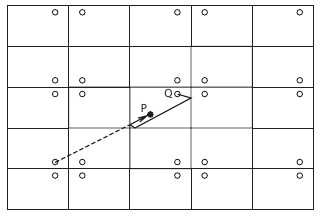
\includegraphics[scale=1]{pics/room1}
\caption{Замощение плоскости отражёнными копиями комнаты.}
\label{pic:room1}
\end{figure}

На полученной картинке каждый выстрел представляется отрезком от какой-то копии точки $Q$ до точки $P$.
Каждый раз, когда такая линия пересекает границу между прямоугольниками, лазерный луч отражается от стенки.
На рисунке показана одна из таких (пунктирных) линий; сплошная линия --- это путь соответствующего луча.

Нам надо перехватить любой выстрел.
Для этого сделаем копию плоскости, показанной на рис. \ref{pic:room1}, прикрепим её к плоскости в точке $P$, и уменьшим эту копию вдвое по вертикали и горизонтали.
Копии точки $Q$ на уменьшенной плоскости будут подходящими позициями охранников.
Они выполняют свою задачу, ведь они лежат ровно на полути между копиями пушки исходного замощения и вами.

На рис. \ref{pic:room2} уменьшенная копия изображена серым цветом, и указаны некоторые воображаемые пути лазера; можно видеть, что на полпути они проходят через соответствующие более мелкие точки серой сетки.

\begin{figure}[t!]
\centering
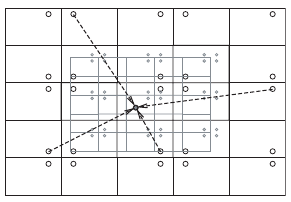
\includegraphics[scale=1]{pics/room2}
\caption{Уменьшенная копия плоскости с точкой $P$ наложенной на себя.}
\label{pic:room2}
\end{figure}

\begin{figure}[b!]
\centering
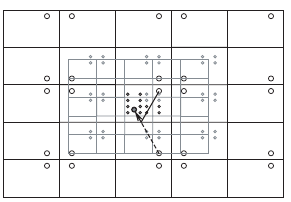
\includegraphics[scale=1]{pics/room3}
\caption{Позиции телохранителей в исходном прямоугольнике.}
\label{pic:room3}
\end{figure}

Конечно, таких точек бесконечно много, но мы утверждаем, что все они являются отражениями набора из 16 точек в исходной комнате.
Четыре из них уже находятся в исходной комнате.
Четыре точки в комнате слева от исходной можно отразить обратно, получив четыре новые точки; аналогично для комнаты выше исходной.
Наконец, четыре точки в комнате \emph{выше и слева} от исходной комнаты могут быть отражены дважды, и так мы получим последние четыре точки в исходной комнате.
На рис.~17 к исходной серой четвёрке точек добавлены двенадцать новых чёрных,
а также показан воображаемый путь лазера и его настоящий путь, проходящий через одну из новых точек.

Поскольку каждая комната выглядит точно так же, как и исходная, или одна из трёх других, которые мы только что рассмотрели, все позиции охранников в плоскости являются отражениями описанных шестнадцати точек в исходной комнате.
Поскольку каждая линия от копии $Q$ проходит через отражённого охранника, фактический выстрел попадает в поставленного охранника на полпути (если не раньше) и поглощается.

Если выбрать местоположения точек $P$ и $Q$ специальным образом, то позиции некоторых охранников совпадут, но в общем случае потребуется полный набор из шестнадцати.

\begin{addedbytheeditors}
Возможно, проще разобрать сначала задачу на плоском торе (то есть в прямоугольнике со склеенными противоположными сторонами).
Убедиться, что в этом случае достаточно четырёх охранников, а потом свести   задачу про прямоугольник к четырём задачам о торе.

Если вам понравилась задача, попробуйте расставить конечное число охранников произвольно близко к точке $P$.\pr
\end{addedbytheeditors}



\subsubsection*{Ящик в ящике}

Эту замечательную головоломку мне подкинул Энтони Квас (Университет Виктории), который услышал её и приведённое ниже решение от Исаака Корнфельда, профессора Северо-Западного университета (Иллинойс).
Корнфельд узнал о ней много лет назад в Москве.

Пусть $B_\varepsilon$ --- $\varepsilon$-окрестность параллелепипеда $B$;
другими словами, это множество всех точек в пространстве, находящихся на расстоянии $\varepsilon$ или меньше от какой-либо точки $B$.
Если $B$ имеет размеры $a \z\times b \z\times c$, то множество $B_\varepsilon$ выглядит как параллелепипед $(a + 2\varepsilon) \z\times (b + 2\varepsilon) \z\times (c + 2\varepsilon)$ с закруглёнными краями и углами.
Точный объём $B_\varepsilon$ будет равен
$abc$ (объем $B$)
плюс $2ab\varepsilon + 2ac\varepsilon + 2bc\varepsilon$ (объем пластин, добавленных к шести граням)
плюс $4a\pi\varepsilon^2 /4 + 4b\pi\varepsilon^2 /4 + 4c\pi\varepsilon^2 /4$ (объем 12-ти штапиков вдоль рёбер --- каждый с поперечным сечением в виде четверти круга),
плюс $4\pi\varepsilon^3 /3$, так как восемь осьмушек, добавленных к углам, образуют целый шар.
Всего получим
\[V(B_\varepsilon)=\tfrac43\pi\varepsilon^3+(a+b+c)\pi\varepsilon^2+2(ab+bc+ca)\varepsilon+abc.\]

Изобразить $B_\varepsilon$ довольно сложно, поэтому мы спустимся на плоскость;
на рис. \ref{pic:box}, показано как выглядит $B_\varepsilon$ для прямоугольника $B$ размера $a \times b$.
Формула для площади $B_\varepsilon$ будет:
\[S(B_\varepsilon)=\pi\varepsilon^2+2(a+b)\varepsilon+ab.\]

\begin{figure}[ht!]
\centering
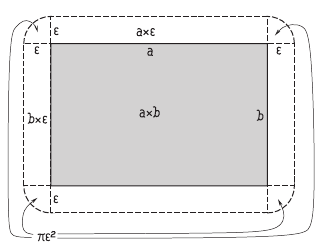
\includegraphics[scale=1]{pics/box}
\caption{$\varepsilon$-окрестность прямоугольник $a \times b$.}
\label{pic:box}
\end{figure}

Вернёмся в трёхмерное пространство.
Если ящик $A$ (с размерами, скажем, $a'\times b'\times c'$) находится внутри ящика $B$, то $A_\varepsilon$ также находится внутри $B_\varepsilon$ для любого $\varepsilon > 0$.
Следовательно, $V(A_\varepsilon ) \z< V(B_\varepsilon)$.
Однако, если выбрать \emph{огромное} $\varepsilon$, то доминирующим членом в разнице их объёмов станет
\[(a+b+c)\pi\varepsilon^2-(a'+b'+c')\pi\varepsilon^2\]
Этот член обязан быть неотрицательным, значит, ящик $B$ дороже чем~$A$.

Эта задача появлялась на Турнире городов 1998 года (5-я задача основного варианта).
Предложенное там решение было другим.
Оно принадлежало Андрею Сторожеву, выходцу из России, который сейчас работает в Австралийском Математическом Фонде.
Решение Сторожева основано на наблюдении, что площадь поверхности внутреннего ящика $A$ должна быть меньше, чем у  $B$.
Это можно увидеть, спроецировав каждую грань $A$ наружу перпендикулярно самой себе и посмотрев на покрытые части поверхности $B$.
Утверждение следует из того, что эти 6 частей не пересекаются, и каждая не меньше соответствующей грани $A$.

Сравнение площадей записывается алгебраически 
\[2a'b'\z+2b'c'\z+2c'a' \z< 2ab\z+2bc\z+2ca\] 
и мы также знаем, что $a'^2\z+b'^2\z+c'^2\z<a^2\z+b^2\z+c^2$, сравнивая диагонали двух ящиков.
Сложив эти два неравенства, получаем 
\[(a'+b'+c')^2<(a+b+c)^2\]
--- готово!

\begin{addedbytheeditors}
Задачу можно воспринимать как рекламу \emph{смешанным объёмам} --- замечательному инструменту в исследовании выпуклых тел.
С ним можно познакомиться по классической книге \cite{burago-zalgaller}.

То, что объём $\varepsilon$-окрестности любого выпуклого тела (не обязательно параллелепипеда) выражается многочленом было замечено Якобом Штейнером \cite{steiner}.
Коэффициенты этого многочлена выражаются через так называемые \emph{поперечные меры}.
Про одномерную поперечную меру можно думать как про среднюю длину проекций тела на случайные прямые.
Двумерная мера --- это средняя площадь проекций на случайные плоскости, и так далее.
Можно думать, что $k$-мерная поперечная мера есть матожидание площади проекции тела на случайное $k$-мерное подпространство.
В $d$-мерном пространстве у выпуклого тела есть поперечные меры всех размерностей от $1$ до $d$;
поперечная мера размерности $d$ --- это объём тела, а $(d-1)$-мерная пропорциональна площади его поверхности.

В любом случае ясно, что если одно тело содержится в другом, то $k$-мерная поперечная мера у первого не больше, чем у второго.
Это даёт серию обобщений нашей задачи на все размерности.

В решении используется, что 1-мерная поперечная мера параллелепипеда пропорциональна сумме его измерений.
Оно было найдено в 1999 году Александром Шенем \cite{shen}, но возможно, было известно и раньше.
Заметим, что то же рассуждение доказывает, что требуемое неравенство выполняется для всех параллелепипедов (не обязательно прямоугольных) --- то есть если один параллелепипед содержит другой, то сумма всех рёбер внешнего не меньше суммы рёбер внутреннего.
В той же статье приводится пара других вариаций этого решения.

В книге~А. К. Толпыго \cite{Tolpygo2010} приводится ещё одно решение
В нём предлагается рассмотреть $9$ чисел~--- длины проекций ребёр внутреннего параллелепипеда на рёбра внешнего.
Во первых, сумма проекций любого ребра не меньше, чем само ребро.
Далее заметим, что сумма трёх проекций на данное ребро внешнего параллелепипеда не превосходит длины этого ребра.
Отсюда видно, что размер внутреннего параллелепипеда не превосходит суммы девяти проекций, которая в свою очередь не превосходит размера внешнего параллелепипеда.
\pr
\end{addedbytheeditors}

%В статье \cite{shen} приведено и другое решение, основанное на вероятностных соображениях (согласно смутным воспоминаниям автора это решение ему рассказал кто-то другой).
%Пусть $X$~---  выпуклое множество в $\mathbb{R}^3$.
%Рассмотрим случайную прямую $\ell$ в $\mathbb{R}^3$. Ортогональная проекция $X$ на $\ell$ является отрезком. Обозначим через $d(X)$ ожидаемую длину этого отрезка.
%Если $X_m$ отрезок длины $m$, то $d(X_m)$ пропорционально $m$, т. е. $d(X_m) =km$ для некоторой константы $k>0$.
%(На самом деле $k =1/2$, но точное значение здесь не имеет значения.)
%Пусть теперь $X$~--- ящик размерами $a\times b\times c$. Для каждой прямой $\ell$ проекция $X$ на $\ell$ имеет длину $p_a + p_b+p_c$, где $p_a$, $p_b$, $p_c$~---  проекции отрезков рёбер коробки с длинами $a$, $b$, $c$ соответственно. Усредняя, получаем, что $d(X) = k(a + b + c).$
%Если ящик $X'$ размерами $a'\times b'\times c'$ находится внутри $X$, то проекция $X'$ на произвольную прямую $\ell$ будет покрыта проекцией $X$ на $\ell$, поэтому $d(X')\le d(X)$.
%Объединив это наблюдение с предыдущим, мы видим, что $a'+b'+c'\le a+b+c.$ 
%А: я закоментил эту часть так как здесь повторялось то, что уже сказано.



